% !TeX root = ../../main.tex
\section{Choice of separator}
A crystallisation system consisting of a melt crystalliser (S104) and a subsequent hydraulic wash column (S106) has been chosen as the appropriate separation technique. A PFD for this system is available in Figure \ref{fig:separator PFD}

%Both units have been modelled to determine appropriate dimensions and evaluate the performance of the units. A sensitivity analysis has been conducted on variables with uncertainty to demonstrate its effect on the designs and the output. Finally, mechanical designs with supplementary CAD drawings of both units are included.

\begin{figure}[h]
    \centering
    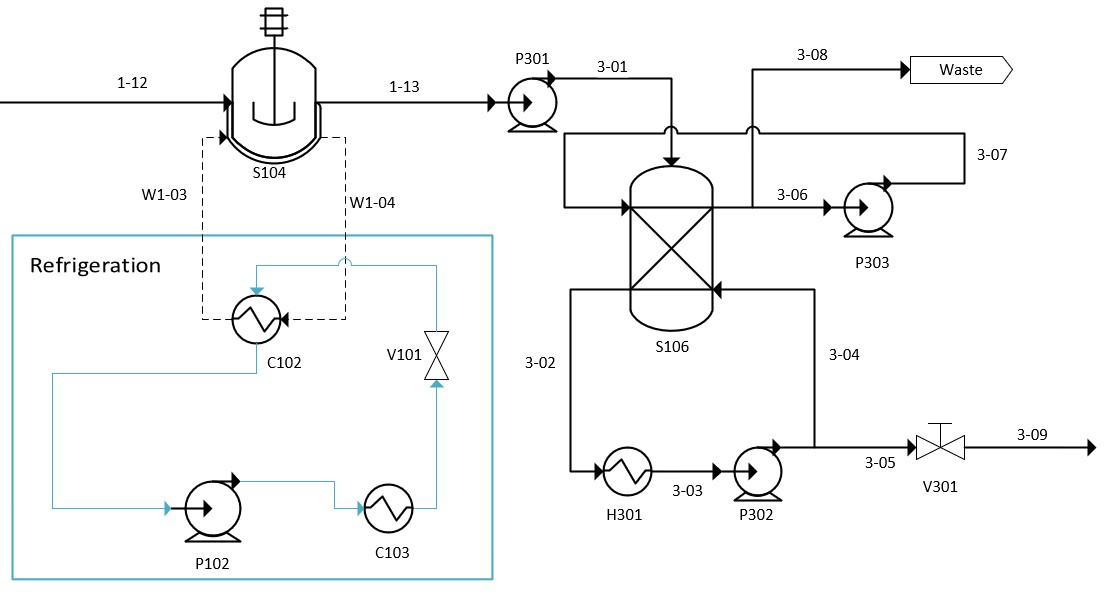
\includegraphics[scale=0.6]{chapters/3-separation/figures/Crystallizer PFD.jpg}
    \caption{PFD of the separation system in consideration; the system consists of a melt crystalliser (S104) and a subsequent hydraulic wash column (S106).}
    \label{fig:separator PFD}
\end{figure}

Due to the small difference in boiling points between nitrotoluene isomers, distillation is infeasible and energy intensive. Similar solubility in both aqueous and organic solvents between the isomers made the use of absorption or adsorption processes infeasible as well. However, crystallisation has been deemed feasible due to the sizeable gaps in melting points between the isomers.

*Table of boiling points, melting points and mole fraction

does not require any additional substances. 

Crystallisation can produce high purity products with very low energy input compared to processes like distillation. The heat of transition in crystallisation is typically two to five times lower than in distillation \cite{noauthor_melt_nodate}. In the industry there are two kinds of process: solution crystallisation and melt crystallisation. Solution crystallisation typically involves the crystallisation of an inorganic solute from aqueous solution; for organics, the solvent utilised could be environmentally-unfriendly, and recovering the solvent or disposing of it could potentially be costly. Melt crystallisation, on the other hand, Melt crystallisers are usually used to separate organic chemicals with favourable melting points, such as in this case. Typically, solution crystallisation consists of the cooling of the mixuture, decrease the components solubility in the solvent. The same effect can also be achieved with antisolvent crystallisation. However In the case of melt crystallisers only solid and liquid phases are involved allowing for smaller volumes which means less capital costs. Compared to solution crystallisers, the growth rate in melt crystalliser is also relatively fast \cite{myerson_handbook_2019}. Therefore, melt crystallisers were found to be more advantageous for separating p-NT from other organic chemicals. 

There are two main types of melt crystallisers present in the industry: solid-layer crystalliser and suspension crystalliser. In solid-layer crystallisers the crystal layer grows perpendicular to a cooled wall into the bulk of a melt known as the mother liquor. It is a multistage purification process. In contrast, suspended melt crystallisers involve crystals freely suspended in the melt. The crystallisation initiates on cooled surfaces and the crystals are scraped off. Therefore, crystal growth occurs on the crystals suspended in the melt \cite{myerson_handbook_2019}. Table \ref{tab:crystallisertype} shows the advantages and disadvantage of the two main crystalliser types discussed. 

\begin{table}
\caption{Comparison of crystallisers \cite{myerson_handbook_2019} }
\label{tab:crystallisertype}
\begin{tabularx}{\linewidth}{@{}lXX@{}}
\toprule
Type & Advantages                 & Disadvantages                               \\ \midrule
Solid layer & \begin{itemize}[label=+,leftmargin=1em]
  \item Avoids encrustation issue 
  \item Controllable crystal growth rate 
  \item No slurry handling, easy to operate
\end{itemize} & \begin{itemize}[label=-,leftmargin=1em]
  \item The surface area is a limiting factor so bigger plant sizes required, high investment costs
  \item Multistage process, increases energy consumption and plant size 
  \item Commonly batch process
\end{itemize} \\\midrule 
Suspension &  \begin{itemize}[label=+,leftmargin=1em]
  \item Moderate crystal growth and large surface areas 
  \item High purity product in one step, less energy consumption
  \item Relatively compact process
  \item Continuous process
\end{itemize} & \begin{itemize}[label=-,leftmargin=1em]
  \item Slurry handling, stirrers required to avoid sedimentation
  \item High purity product in one step so less energy consumption
  \item Encrustation issues 
  \item Solid-liquid separation required, an additional operation cost
\end{itemize}
\\\bottomrule
\end{tabularx}
\end{table}

Even though solid-layer crystallisation has its obvious advantages, the fact that it is a multistage batch process made it unattractive. In suspension crystallisation the surface area for the same volume of crystals is approximately two to three order of magnitude higher than in solid-layer crystallisation \cite{noauthor_types_nodate}. Suspension crystallisation can achieve a high purity in one stage whilst layer crystallisation would require more stages to achieve the same level of purity. Hence, it would consume less energy compared to layer crystallisation. Moreover, Nitroma aims for continuous operation throughout the plant to eliminate dangers from material handling. Suspension crystalliser was more suitable for this purpose. Mixed-suspension mixed-product removal (MSMPR) was chosen. It operates continuously by producing a slurry of p-NT crystals and m-NT liquid.

In order to obtain p-NT at greater than 90 \% purity it has to be separated from m-NT and o-NT. Conventional solid-liquid separators are typically operated in batch or semi-batch.Since Nitroma aims for a continuous plant these separators were not suitable. For instance, a centrifuge would require  solid material handling possibly using a conveyor belt to transport the solid. This has many difficulties and could become a bottle neck in the entire plant. Alternatively, wash columns were considered as they can be operated continuously and achieve ultrapurification. 

